\chapter{Case study: the iTrust SWaT System}
\label{casestudy}

\linenumbers
\lettrine[lines=2]{H}{aving} introduced the innovative framework and highlighted its potential in the preceding chapter, we now turn our attention to the case study where we will apply this framework. As previously mentioned in Chapter \ref{chap:proposal} and demonstrated through various examples in the same chapter, our focus will be on the \textbf{iTrust SWaT system} \cite{swat_home}, developed by the University of Singapore for Technology and Design \cite{itrust_site}. The acronym SWaT represents \textit{\textbf{S}ecure \textbf{Wa}ter \textbf{T}reatment}.

\bigskip
The iTrust SWaT system is a testbed that replicates on a small scale a real water treatment plant arises to support research in the area of cyber security of industrial control systems and has been operational since March 2015: it is still being used by students at the University of Singapore for educational and training purposes and is available to organizations to train their operators on cyber physical incidents.

\section{Architecture}
\label{sec:5_swat_architecture}
In contrast to the virtualized testbed discussed in Section \ref{subsec:ceccato_testbed} by Ceccato et al., the iTrust SWaT system is composed entirely of physical hardware components. It encompasses various elements, starting from field devices and extending to PLCs, HMI, SCADA workstations, and the SCADA server (also referred to as the \textit{historian}). The historian is responsible for recording data from field devices for further analysis. In the upcoming sections, we will delve deeper into the architecture of the physical process and the communication network.

\subsection{Physical Process} 
\label{subsec:5_swat_physical_architecture}
The physical process of the SWaT consists of six stages, denoted P1 through P6. These stages are \cite{swat_tecnical_pdf}\cite{swat_tippenhauer}:

\begin{enumerate}
	\item \textbf{taking in raw water:} feeds unfiltered water into the system
	\item \textbf{chemical dosing:} adds chemicals to water useful for initial pretreatment
	\item \textbf{Ultra Filtration (UF) system:} the water is filtered through a semi-permeable membrane (ultrafiltration membrane) using the liquid pressure, effectively capturing impurities and suspended solids, as well as removing bacteria, viruses, and other pathogens present in the water.
	\item \textbf{dechlorination:} removes residual chlorine from disinfected water using ultraviolet lamps
	\item \textbf{Reverse Osmosis (RO):} performs further filtration of the water
	\item \textbf{backwash process:} cleans the membranes in UF using the water produced by RO
\end{enumerate}
Figure \ref{fig:5_swat_architecture_1} shows a graphical representation of the architecture and the six stages of the SWaT system.

\begin{figure}[ht]
	\centering
	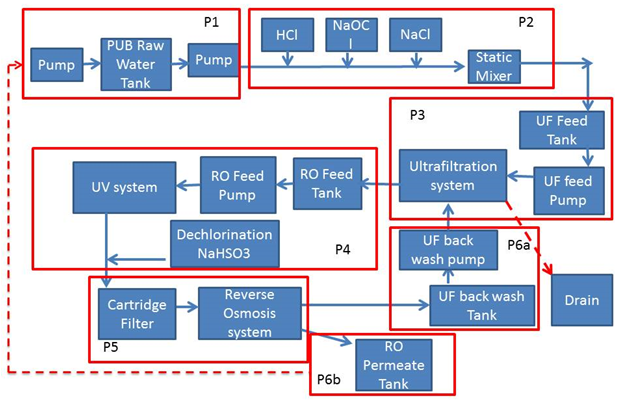
\includegraphics[scale=0.55]{chap5/testbed-3.png}
	\caption{SWaT architecture}
	\label{fig:5_swat_architecture_1}
\end{figure}

\bigskip
The SWaT system incorporates an array of sensors that play a crucial role in monitoring the system's operations and ensuring their safe. These sensors are responsible for continuously collecting data and providing valuable insights into the functioning of the system. These sensors are:

\begin{itemize}
	\item Level Indication Transmitter (measured in mm)
	\item Flow Indication Transmitter (m3/hr)
	\item Analyser Indicator Transmitter
	\begin{itemize}
		\item[o] Conductivity (µS/cm)
		\item[o] pH
		\item[o] Oxidation Reduction Potential (mV)
	\end{itemize}
	\item Differential Pressure Indicator Transmitter (kPa)
	\item Pressure Indicator Transmitter (kPa)
\end{itemize}
The sensors and actuators associated with each PLC are shown in Figure \ref{fig:5_swat_sensors_plc}. \newline
Sensors and actuators are mapped to tags by the communication protocol used (see \ref{subsec:5_swat_network_architecture}): a tag can be addressed via string descriptor defined by the system designer (e.g. MV101, to indicate motorized valve number 1 at stage 1) or by referring directly to the analog/digital pins of the PLC I/O unit \cite{swat_tippenhauer}.

\begin{figure}[ht]
	\centering
	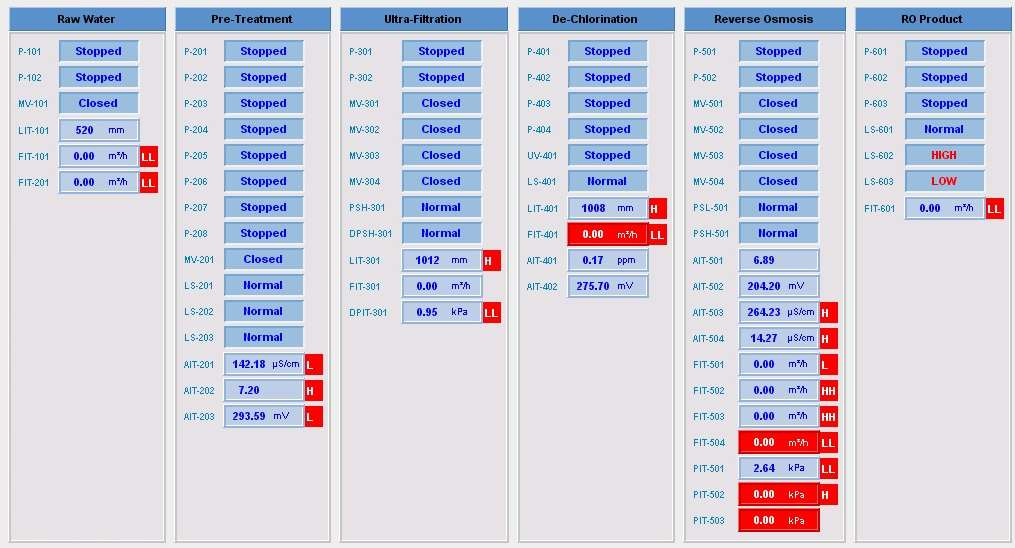
\includegraphics[scale=0.50]{chap5/plc-devices.jpg}
	\caption{Sensors and actuators associated with each PLC}
	\label{fig:5_swat_sensors_plc}
\end{figure}

\subsection{Control and Communication Network}
\label{subsec:5_swat_network_architecture}
The SWaT system's network architecture follows the principles of layering and zoning, which enable segmentation and control of traffic within the network.
\newline \newline
Five layers are present starting from the highest to the lowest: 

\begin{itemize}
	\item \textbf{Layer 3.5} -- Demilitarised Zone (DMZ)
	\item \textbf{Layer 3} -- Operation Management (Historian)
	\item \textbf{Layer 2} -- Supervisory Control (Touch Panel, Engineering Workstation, HMI Control Clients)
	\item \textbf{Layer 1} -- Plant Control Network (PLCs) (Star Network)
	\item \textbf{Layer 0} -- Process (Actuator/Sensors and Input/output modules) (Ring Network)
\end{itemize}
PLCs at Layer 1 communicate with their respective sensors and actuators at Layer 0 through a conventional ring network topology based on EtherNet/IP, to ensure that the system can tolerate the loss of a single link without any adverse impact on data or control functionality.\newline
PLCs between the different process stages at Layer 1 communicate with each other through a star network topology using the CIP protocol on EtherNet/IP, previously discussed in Section \ref{subsubsec:cip}.

\bigskip
Regarding zoning, the SWaT system is divided into three zones, each containing one or more layers. These zones are, in descending order of security level: 

\begin{itemize}
	\item \textbf{Plant Control Network}, or \textbf{Control System:} includes layers from 0 to 2
	\item \textbf{DMZ:} includes Layer 3.5
	\item \textbf{Plant Network:} includes Layer 3
\end{itemize}
Figure \ref{fig:5_swat_network_arch} provides a clearer visualization of the zoning and layer division within the network architecture of the SWaT system. This diagram highlights the distinct zones and their corresponding layers, offering a comprehensive overview of the system's network structure.

\begin{figure}[ht]
	\centering
	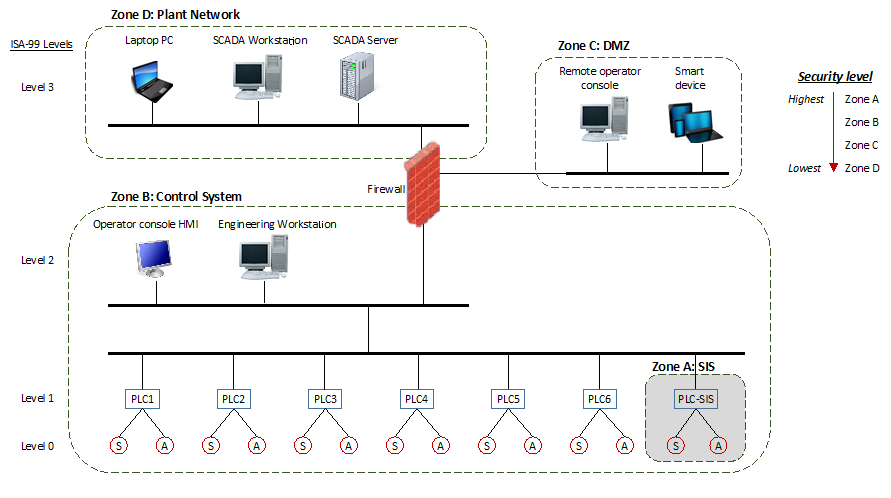
\includegraphics[scale=0.60]{chap5/testbed-4.png}
	\caption{SWaT network architecture}
	\label{fig:5_swat_network_arch}
\end{figure}

\section{Datasets}
\label{sec:5_swat_datasets}

\vfill
\nolinenumbers